% !TEX root = mythesis.tex

%==============================================================================
\chapter{Experimental equipment}
\label{sec:LHCATLAS}
%==============================================================================

\mynote[inline]{}{Write about what the chapter has to offer}


\section{The Large Hadron Collider}
The Large Hadron Collider (LHC)\cite{LyndonEvans_2008} is a two-ring proton-proton collider situated near Geneva across the Swiss-French border. It is built in 
the 26.7 km long tunnel that previously housed the Large Electron-Positron (LEP) collider. The two proton beams are accelerated in opposite directions and 
brought into collision at four points where the four detectors are located. The LHC has two transfer tunnels of 2.5 km each that connects to the CERN accelerator
complex as shown in \cref{fig:acc_complex}. 

The CERN accelerator complex is a set of subsystems that contribute to the acceleration of protons. The process 
starts with negative Hydrogen ions that are accelerated in LINAC4 which is the first system in the CERN accelerator complex. Electrons are stripped off from 
Hydrogen ions during injection from LINAC4 to Proton Synchrotron Booster (PBS) which increases the proton energy further. Eventually the protons are fed into 
the Super Proton Synchrotron (SPS). At this point the proton energy is 450 GeV and then they are finally injected into two opposing beams of the LHC. Here each beam 
attains a path-breaking energy of 6.5 TeV. 

\begin{figure}[htbp]
    \centering
    \includegraphics[width=\figwidth]{Poster-2013-377.jpg}
    \caption[Sketch of the CERN accelerator complex]{Sketch of the LHC ring along with the machines in the CERN accelerator complex\cite{Haffner:1621894}.}%
    \label{fig:acc_complex}
\end{figure}

\subsection*{Superconducting magnets}
One of the major challenges at the LHC is the directing of proton beams along the circular structure. To achieve the destined center of mass energy, 
given the circumference and charge of proton, approximately 8 T magnetic field is required. This is outside the limit of conventional magnets which is why 
superconducting magnets are engaged. Due to the limited available area in the LHC tunnel, a single magnet system is shared by both the beam pipes. The 
superconducting coils are immersed in a superfluid Helium bath which is cooled down to a certain low temperature to achieve superconductivity. One of the 
obstacles here is the synchrotron radiation. The protons radiate photons when they are accelerated and this radiation can adversely impact the temperature 
inside the magnet system. To fix this problem, beam screens are placed between the beam pipe and the magnet system which reflects or absorbs these radiated photons,
preserving the superconductivity. 

\subsection*{Luminosity and cross-section ($\sigma$)}
The quantity that measures the ability of a collider to produce particle interactions is called
instantaneous luminosity ($\mathcal{L}$). The instantaneous luminosity integrated over the lifetime
of collider operation is called integrated luminosity ($L$).

In order to define the event rate for interesting processes, along with luminosity, we require
another quantity called the cross-section. At the subatomic scale, the particle interactions 
are governed by laws of quantum physics. Therefore, a theory can predict 
the \textit{probablility} of certain outcomes of collisions. The probablity that a certain
process will take place is called its cross-section ($\sigma$). Finally, the number of event rate of
specific interactions is defined as the product of integrated luminosity and the cross-section (\cref{eq:lumi}).
\begin{equation}
    R = \sigma \cdot \int_{dt} \mathcal{L}(t)
    \label{eq:lumi}
\end{equation}

For a particle collider, beam energies and the luminosity are two important figures of merit. 
High energy allows the production of new heavy particles and high luminosity allows more flux 
of particles contributing to high number of collisions. 

At the LHC, the incoming protons see each other as a bunch of partons instead of a single 
proton. The proton is composed of two $u$- and one $d$- quark called valence quarks. At high 
energies, these quarks can exchange gluons and in turn produce more gluons and quarks. In a way,
the proton looks like a \textit{sea} of gluons and quarks that altogether are called partons. 
Here the net flavour of a proton is the same as that of valence quarks. These partons interact 
at collision points and give rise to different SM processes.

The outcomes of these collisions hold interesting physics and it is studied with the help of particle detectors. The LHC houses four main detectors at the four collision
points. The two general purpose detectors are ATLAS (\textbf{A} \textbf{T}oroidal \textbf{L}HC \textbf{A}pparatu\textbf{S})\cite{TheATLASCollaboration_2008} and
CMS (\textbf{C}ompact \textbf{M}uon \textbf{S}olenoid)\cite{TheCMSCollaboration_2008}. The LHCb experiment\cite{TheLHCbCollaboration_2008} is dedicated to 
studies based on \PB-hadron and its decays whereas ALICE(\textbf{A} \textbf{L}arge \textbf{I}on \textbf{C}ollider \textbf{E}xperiment)\cite{TheALICECollaboration_2008}
analyses the $Pb$-$Pb$ collisions at the LHC. This analysis uses data from the ATLAS detector
which is described in the next section. 


\section{The ATLAS detector}
The ATLAS detector is one of the general purpose detectors at the LHC. It is an assembly of sub detectors constructed around the beam pipe in an onion-shaped structure as shown
in \cref{fig:atlas}.

\begin{figure}[htbp]
    \centering
    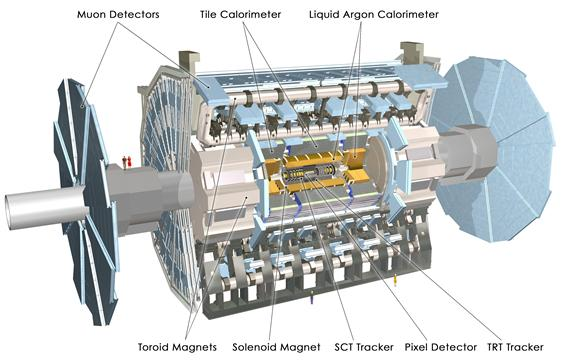
\includegraphics[width=\figwidth]{atlas_layout.jpg}
    \caption[Overview of the ATLAS detector]{An overview of the ATLAS detector\cite{Pequenao:1095924}.}%
    \label{fig:atlas}
\end{figure}

\subsection{Coordinate system}
ATLAS uses a conventional coordinate system in which the point where collisions occur, called the Interaction Point (IP), is treated as the origin. The 
$z$-axis is along the beam direction, $x$-axis is directed to the center of the LHC ring and the $y$-axis is pointing upwards. The azimuthal angle ($\phi$) 
is the angle with the $x$-axis (around the beam pipe) and the polar angle ($\theta$) is the angle from the $z$-axis (from the beam pipe). A sketch of the coordinate
system is shown in ~\cref{fig:coordinatesys}. It is crucial to note that the colliding protons are traveling along the beam direction and given this coordinate 
system, the boosts parallel to the $z$-axis are 
taken into account. This leads to the definition of rapidity as follows:

\begin{equation*}
    y = \frac{1}{2}\text{ln} \Bigl(\frac{E+p_zc}{E-p_zc}\Bigl)
\end{equation*}


If a collided particle is highly relativistic and launched almost perpendicular to the $z$-axis, its $p_z$ will be close to zero leading to zero rapidity.
Another scenario would be that the particle is moving along the $z$-axis and in that case the rapidity will be $\pm \infty$. For large
collider experiments precise calculation of $E$ and $p_z$ is difficult and therefore, a quantity called pseudorapidity is used. It is conceptually similar to 
rapidity and is defined as:

\begin{equation*}
    \eta = -\text{ln} \text{tan}\frac{\theta}{2}
\end{equation*}

\begin{figure}[htbp]
    \centering
    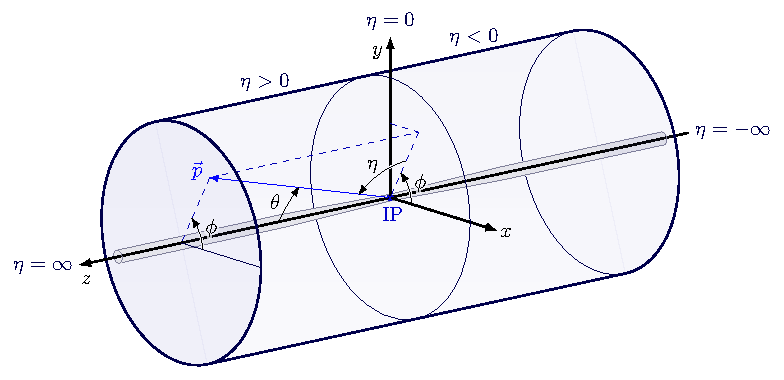
\includegraphics[width=\figwidth]{coordinate_system.pdf}
    \caption[Sketch of the ATLAS coordinate system]{Sketch of the ATLAS coordinate system. Based on \cite{coordinatesys}.}%
    \label{fig:coordinatesys}
\end{figure}

\subsection{The Inner Detector}
The closest sub detector system from the beam pipe is the Inner Detector (ID). It has a cylindircal barrel region covering $|\eta|<1$ and two end-cap regions covering 
$1 \leq \eta \leq 2.5$~\cite{BARBERIS2000331}. The ID comprises of the Pixel Detector, the Semiconductor Tracker (SCT) and the Transition Radiation Tracker (TRT) immersed in a 2 T solenoidal 
magnetic field. Data recorded by these components are used to reconstruct charged-particle trajectories which eventually are used to measure momenta of particles. 

The Pixel Detector resides along the innermost radii of 33-150 mm~\cite{Aaboud_2017}. Modules of silicon pixels are arranged in three layers in the barrel region and two layers in the end-cap region. 
It provides a three-dimensional space-point reading that allows for the reconstruction of primary and secondary vertices. The high granularity of these pixels provide high spatial 
resolution that is beneficial in pattern recognition. The next sub component is the Semiconductor Tracker (SCT) which consists of silicon microstrip detectors 
arranged in four barrel layers and two end-cap layers. The radii range of the SCT is 299-560 mm. The outermost sub component is the Transition Radiation Tracker (TRT) which 
is made up of gaseous straw tube detectors. It spans across 563-1066 mm radii. The straws are filled with xenon and carbon-dioxide at atmospheric pressure and each straw
has a gold-plated tungsten wire along the longitudinal axis. The transition material is a low-density foam surrounding the straws. Tracks of particles are reconstructed from TRT
data. A combination of measurements given by the sub components help get a high-resolution vertex and momentum measurement of
incoming particles. 

\subsection{Calorimeters}
Detector system surrounding the ID are calorimeters. The tasks of a calorimeter include accurately measuring energies and position of incident
particles. The particles emerging after a certain process during collisions, interact with the active material inside the calorimeters and produce secondary particles. The incoming
particle loses almost all its energy inside the calorimeter by producing a shower of secondary particles. These showers are read-out and recorded for accurate energy measurements. 
Besides a decent area coverage, sufficient depth is also an important parameter for calorimeters. In order to contain the showers, calorimeters at ATLAS are designed such that they cover a 
full $\phi$-range and $|\eta|<4.9$.  

\subsection*{Electromagnetic Calorimeter (ECAL)}
The Electromagnetic Calorimeter (ECAL) is a lead-liquid-argon calorimeter split into a barrel component ($|\eta|<1.475$) and two end-cap components 
($1.375 < |\eta| < 3.2$)~\cite{TheATLASCollaboration_2008}. Over the precision physics $\eta$ region, essentially the region coinciding with the inner detector, there are highly granular
detectors capable of accurately measuring electron energies. The ones outside this range are coarser but still adequate for jets and missing transverse energy measurements.
The ECAL is a sampling detector in which liquid argon (active material) and lead absorbers are placed alternatively in an accordian geometry. This geometry allows for a full 
$\phi$-coverage. 

The incident particles encounter the absorber, producing charged particles that ionise the argon atoms. The resulting electrons travel towards the electrodes and a
signal is recorded. The depth of the ECAL is decided according to the radiation length. The radiation length $X_0$ is a characteristic of a material which is defined as 
the length at which the energy of a particle traversing the material, is reduced by a factor of $1/e$. The thickness of ECAL is $> 22 X_0$ in the barrel and $> 26 X_0$ in the end-cap
regions. The energy resolution of the ECAL is $\sigma_E/E = 10\%/\sqrt{E} \oplus 0.7\%$~\cite{CERN-LHCC-2017-018}.

\subsection*{Hadronic Calorimeter (HCAL)}
The Hadronic Calorimeter (HCAL) consists of the tile calorimeter, the Hadronic End-Cap calorimeter (HEC) and the Forward Calorimeter (FCal). The tile calorimeter~\cite{Francavilla_2012} is of a sampling
type, covering a range of $|\eta|<1.7$. The active material consists of iron and plastic, absorbers are made of steel and wavelength shifting fibers are used for readout.
Readout cells are defined by grouping certain number of fibers onto the same Photo Multiplier Tube (PMT). 

Overlapping some $\eta$ region of the tile calorimeter, there is the HEC which occupies
$1.5 < |\eta| < 3.2$. It is a copper-liquid-argon sampling calorimeter consisting of two independent wheels per end-cap situated right behind the end-cap electromagnetic
calorimeters. The detector responsible for detecting large $|\eta|$ objects is the FCal which has a coverage of $3.1 < \eta < 4.9$. The active material (liquid-argon) is 
placed in smaller gaps between the electrodes compared to the gaps in the ECAL. The reason is to avoid ion build-up problems caused by the heavy particle flux 
encountered by the FCal. Forward calorimetery is essential to increase the detection of high momentum jets that would otherwise escape detection at low 
$\eta$~\cite{J-P-Archambault_2008}. It allows a hermetic calorimetry that leads to efficient missing $\text{E}_\text{T}$ measurements. The resolution of the tile 
calorimeter and HEC is $\sigma_E/E = 50\%/\sqrt{E} \oplus 3\%$ while the FCal has a resolution of $\sigma_E/E = 100\%/\sqrt{E} \oplus 10\%$~\cite{A-Artamonov_2008}.
 


\subsection{Muon spectrometers (MS)}
The muon spectrometers play a significant role in accurate measurements of high energy muons. The structure is made up of three superconducting toroids, 
precision tracking chambers and the trigger system. The Barrel toroid is made of eight superconducting coils, having a coil area of $5 \times 26 \text{m}^2$ each 
providing a magnetic field in the range of 0.5 to 2 T. In the end-cap region, eight superconducting coils are situated inside an insulation vessel, providing magnetic 
field in the range 1 to 2 T~\cite{Palestini:2003noa}. 

The hunting of muon candidates from the collided particles is done by the ATLAS muon trigger. It comprises of the Level-1 muon trigger and the High-Level muon trigger implemented with 
different detectors. The Resistive Plate Chambers (RPCs) are placed in the Barrel region and the Thin Gap Chambers (TGCs) are placed in the end-cap region. Different types of 
detectors are used in barrel and end-cap because the muon flux encountered by these regions is different. 

The RPCs and TGCs form the so-called Level-1 muon trigger. It selects muon
candidates with high $p_T$ by reconstructing tracks that point directly towards the interaction point. The precision tracking 
chambers house the Monitored Drift Tubes (MDT) that perfrom the precision measurement of muon momentum. Each chamber
contains two layers, each formed by three or four more layers of drift tubes. The drift tubes are made up of aluminium and are filled with $\text{Ar}-\text{CO}_2$ gas mixture.
The MDTs along with Cathode Strip Chambers (CSCs) form the High-Level muon trigger. Both these triggers operate based on a preconfigured threshold value. In Run-2, for high-$p_T$ the 
threshold was 20 GeV for Level-1 muon trigger and 26 GeV for High-Level muon trigger.  

\subsection{Magnet system}
The ATLAS detector is exposed to large flux of decay products during its operation. A strong magnetic
field is required to bend the paths of charged particles for momentum measurements. For this purpose,
a highly efficient magnet system including a central solenoid, barrel toroidal and two end cap toroidal
magnets. The central solenoid magnet, operating with a current of 7.6 kA, is wrapped around the beam
axis and provides a 2 T magnetic field to the Inner Detector. The barrel and end cap toroidal magnets
operate at 20.5 kA and provide a magnetic field ranging from 0.5 to 1 T in the muon chambers. The
barrel toroidal magnet is built from eight coils and kept equi-spaced to form a toroid-shaped magnet.
The end cap magnets are placed inside the barrel toroidal magnet at both ends of the central solenoid
magnet.

\subsection{Trigger and Data Acquisition System}
The Trigger and Data Acquisition system (TDAQ) has two components, the data acquisition system which reads data
from the detector subsystems and the trigger system which decides which data to retain.
 
ATLAS uses a two-staged trigger system formed by the Level-1 (L1) trigger and the High-Level Trigger (HLT)~\cite{The-ATLAS-collaboration_2020}. The
L1 trigger is a hardware based trigger that selects meaningful signals from the detector components and passes on 
to the HLT which then performs sophisticated algorithms to only retain interesting physics objects 
which are further stored for offline analysis. The event rate drops from 40 MHz to 100 kHz after the L1 trigger and 
it further drops to 1 kHz after the HLT.

The L1 trigger is composed of L1Calo, L1Muon, L1Topo and Central Trigger Processors (CTPs). The L1Calo processes
signals from the calorimeters whereas L1Muon processes signals from the RPCs and TGCs in the muon spectrometers. 
In order to avoid particles not originating from the interaction point, L1Muon follows coincidence requirements 
based on the inner detector and the calorimeter signals. L1Topo which was an upgrade introduced in Run-2, calculates
event topological quantities of L1 objects, such as the sum of transverse momenta of jets~\cite{Nakahama_2015}. The final decision of 
whether to keep an event or discard it, is made by the CTP in $2.5 \mu s$. It also determines Regions of Interest (RoIs)
to be investigated by the HLT.

The HLT is a software based trigger that applies a typical reconstruction algorithm at a preliminary stage 
followed by more advanced, CPU-intensive algorithms to trigger on events. A farm of CPUs are running several
algorithms in parallel to process signals based on selection criteria similar to offline physics requirements~\cite{C-Gabaldon_2012}.   



\section{Physics objects reconstruction}

The various decay products from the proton-proton collisions travel through the detector volume leaving
behind characteristic trails. Physicists follow the trails and try to reconstruct objects which would represent
characteristics of particles.

At the LHC 2808 bunches of protons are injected which are 25 ns apart. This results into 
$1.2 \times 10^{11}$ protons ber bunch giving rise to many different particle interactions. The 
primary hard scatter collisions, that are of interest, are contaminated by soft interactions 
called pileup. It is defined by the average number of interactions
recorded per bunch crossing. Sources of pileup are categorized into in-time and out-of-time pileup. In-time pile up is due to collisions
occurring in the same bunch-crossing and out-of-time pile-up is contributed by the collisions from previous
or later bunches. Some of the sub-detectors have sensitivity windows longer than the interval between
bunch crossings. This eventually affects the recorded number of interactions per bunch. The accurate
detection of objects under study becomes difficult due to pile-up events. The higher the 
luminosity, more the pileup. The object reconstruction algorithms have dedicated procedures 
to mitigate pileup.
\mynote[inline]{}{Pileup info can be polished}
\subsection{Tracking}
The signals collected from the tracking detectors, the inner detector and muon spectrometers, are used to reconstruct charged-particle trajectories called tracks. The primary-tracking
reconstruction from the SCT and pixel detector is performed in three steps: clusterisation, iterative combinatorial track finding and ambiguity solving~\cite{Aaboud_2017}. 

In the first step, energy deposits which are above the predefined threshold are collected from the pixels and strip detectors. These clusters are used to create
three-dimensional space points that indicate the coordinates of the charged particle's trajectory. A linear approximation tenchique is used to find the intersection
point of a particle on the pixel sensor. In a crowded environment, it may happen that the reconstructed cluster has energies from multiple particles. Therefore,
it is essential for the algorithms to identify such clusters. 

Track seeds are formed using a group of space points. These preliminary track seeds pass through a number of selection criteria to ensure purity. For instance, there should be atleast one 
additonal space point compatible with the track trajectory estimated from the seed. The task of combining the filtered track seeds to construct track candidates is performed by 
the Kalman filter. In principle, it searches for additonal space points from other layers of pixels that are suitable with the track seed. If the filter finds more than one suitable space 
point on the same layer then it creates multiples track candidates per seed. The Kalman filter is also effective in reducing the amount of track candidates from random space points. 

Once all the track candidates are ready, the ambiguity solver is employed. It is required to rectify cases where space points might overlap or have been incorrectly assigned. 
The ambiguity solver processes track candidates individually based on their scores. Each track gets a score based on how likely it is to be a primary reconstructed track. 
It also resolves issues where a cluster is assigned to multiple track candidates. Moreover, track caandidates are rejected if they fail to meet basic track quality requirements based on
minimum transverse momentum, mimimum $|\eta|$ and number of pixels contributing to the cluster formation.

The track candidates that pass the ambiguity solver are used as input to find suitable TRT measurements. The so-called space points in TRT are expressed in $r-\phi$
and $r-z$ coordinates in the barrel and end-cap region respectively. These space points or \textit{hits} are employed by the extension algorithm which performs
a line fit to find hits suitable with the input track candidates. In this way, the chosen hits form the TRT further extend the track candidate~\cite{T_Cornelissen_2008}.

\subsection{Vertexing}
Vertexing is the process of identifying vertices, which are the locations in the detector where proton-proton hard scattering occurs.
Primary vertex is the position where the initial interaction took place whereas secondary vertices
are positions where particles produced in the initial interaction decay.

The vertex reconstruction algorithm takes tracks estimated from the Inner Detector (ID) as input. These tracks are filtered based on certain quality requirements to ensure 
they are suitable for vertex reconstruction. The algorithm operates in two steps: vertex finding and vertex fitting. Initially, a seed position is determined from the set of 
filtered tracks. Then, the seed and the filtered tracks are used to fit the best vertex position. This process is iterative, starting with equal weights for all tracks. As iterations 
progress, the weights of more compatible tracks increase, while those of less compatible tracks decrease. Eventually, the less compatible tracks are returned to the pool for potential 
use in other vertex reconstructions. A vertex candidate must have at least two associated tracks. This procedure is repeated until there are no unassociated tracks left or no more 
vertices can be found from the remaining tracks. The vertex reconstruction algorithm produces a set of three-dimensional vertex positions and their covariance 
matrices~\cite{F_Meloni_vertex}.

The ATLAS reconstruction defines the hard-scatter primary vertex as the primary vertex with the
largest $\sum p_{\text{T}}^2$ of the associated tracks. The other primary vertices are associated
with pileup contribution. 

\subsection{Topo clusters}
Topoclusters, as the name suggests, are topological energy clusters produced inside the calorimeter cells caused by particle showers. 
The technique of collecting calorimeter signals from topologically connected cells and grouping them into clusters is an effective way to extract signal in 
highly granular calorimeters such as the one in ATLAS. It is important to suppress the signals from background noise and pileup contributions and therefore, 
a quantity called signal significance is used to decide which signals contribute to cluster formation~\cite{Aad:2138166}. It is defined as the ratio of the cell signal to the average 
expected noise in this cell. Both these quantities are defined at the electromagnetic scale (EM). The significance is described in \cref{eq:toposigni}.

\begin{equation}
    \varsigma_{\text{cell}}^{\text{EM}} = \frac{E_{\text{cell}}^{\text{EM}}}{\sigma_{\text{noise,cell}}^{\text{EM}}}
    \label{eq:toposigni}
\end{equation}

The topo clusters are seeded and expanded on the basis of some threshold requirements of $\varsigma_{\text{cell}}^{\text{EM}}$. 
The calorimeter cells having $\varsigma_{\text{cell}}^{\text{EM}}>4$ are chosen to be the seeds for topoclusters. Then, the 
neighboruring cells satisfying the requirement of $\varsigma_{\text{cell}}^{\text{EM}}>2$ are added to the seeds and eventually the
cluster grows.

\subsection{Particle Flow}
\label{sec:pflow}
The momentum and energy measurements from the inner detector and calorimeter,respectively, are prone
to overlaps of certain events. For instance, an event in which an electron leaves a track in the ID and also
deposits energy in the calorimeter. If information from these sub detectors is used individually, there is a
possibility of double counting this event. In order to remove such overlaps and to utilize the sub detectors to
the best of their potential, Particle Flow has been developed. The idea of particle flow is to reconstruct an
event by combining measurements from the inner detector and calorimeters. The ID is pileup resilient and
has a better resolution especially at low pT whereas the calorimeter can detect neutral particles. Particle
Flow puts both these advantages into yielding more reliable measurements.

In the Particle Flow (PFlow) algorithm, one of the inputs is the set of reconstructed tracks that are extrapolated
in the direction of calorimeter energy deposits. The algorithm evaluates the probablility of the particle
energy to be depoisted in more than one topocluster. Accordingly it either stores single topocluster energy
or sums up energy of multiple topoclusters to constitute the full energy profile of the particle that created the
track. The expected energy deposited by the particle that created the track is subtracted from the matched
topoclusters. The remaining energy after subtraction is compared to a threshold value. If the energy is below the 
threshold, it is removed as it may be due to shower fluctuations. Conversely, if the energy exceeds the threshold, 
it is retained as it may originate from multiple particles. At the end, a set of selected tracks and remaining
topoclusters in the calorimeters represent the reconstructed event with no double counting of signatures. A schematic 
diagram of PFlow algorithm is shown in \cref{fig:pflow}.

\begin{figure}[htbp]
    \centering
    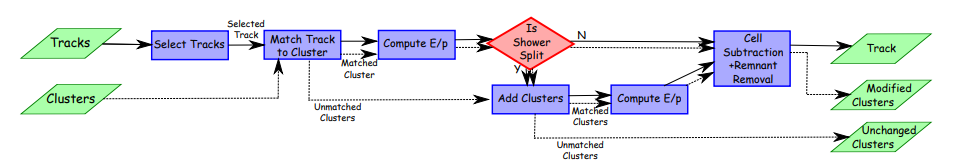
\includegraphics[width=\figwidth]{pflow.png}
    \caption[Particle flow overview]{A chart representing the Particle Flow algorithm~\cite{Aaboud:2257597}}%
    \label{fig:pflow}
\end{figure}

\subsection{Charged particles}
\subsection*{Electrons}
The topoclusters from the electromagnetic calorimeter and the charged particle tracks from the inner
detector are used to reconstruct an electron candidate. The procedure is divided into three steps:
\begin{itemize}
    \item A sliding-window algorithm is used to identify seed clusters that exceed a transverse
    energy of 2.5 GeV. The algorithm scans the area in either $\eta$ or $\phi$ to locate seed clusters. 
    \item The reconstructed tracks in the inner detector that loosely match with the seed clusters
    are selected and a fitting procedure is applied. The separation of the cluster-center and the 
    track must fulfill $|\eta_{\text{cluster}} - \eta_{\text{track}}|<0.05$
    \item A tight matching of fitted tracks and seed clusters is performed. The requirements are based
    on the proximity criteria such as the track matching in $\phi$ is allowed to be $-0.10< \Delta\phi <0.05$.
\end{itemize}

If multiple tracks fulfill the matching criteria, additional requirements are imposed to select the 
primary electron track. One of these requirements is that the chosen track should not have any association with 
a vertex from a photon conversion~\cite{Aaboud_2019}. 

\subsection*{Muons}
There are two types of muon reconstruction algorithms: stand-alone reconstruction from the MS and global
reconstruction based on signals from the MS and the ID. 

Under the stand-alone method, track segments are identified from different MS stations using Hough transform.
By combining these segments, basic track candidates are constructed. Then a global-$\chi^2$ fit of the 
muon trajectory through the magnetic filed is performed and based on the fit results, unsuitable hits are
removed. Moreover, hits that were not considered before are now added and the fit is re-performed. 
In the ambiguity resolution step, tracks that share a large number of high-quality hits. 

The global reconstruction of muons is performed based on the information from the ID and the MS, along
with energy loss inside the calorimeters. There are five different strategies leading to different
muon types:
\begin{itemize}
    \item Combined muon (CB): Here a combined track fit is performed on the hits extracted from both
    the tracking sub detectors. Moreover, calorimeter energy loss is also considered. 
    \item inside-out muon (IO): The ID tracks are extrapolated to the ID and at least three loosely
    alligning MS hits are obtained. After that, a combined fit is performed on the ID tracks, MS hits
    and calorimeter energy loss. 
    \item Muon-extrapolated (ME): The muons tracks that do not match with any ID tracks are defined for
    a ME muon. These muons are outside the acceptance range of the ID but still in the acceptance range of the
    MS. 
    \item Segment-tagged (ST): The ID tracks are required to match at least one MS segment by fulfilling
    tight angular matching. The ID tracks matched in this way are considered for a muon candidate.
    \item Calorimeter-tagged (CT): Here the ID tracks are extrapolated to the calorimeters to find
    clusters consistent with a minimum-ionising particle. The matched ID track is considered for a 
    muon candidate. 
\end{itemize}


\subsection*{Jets}
Jet reconstruction inputs are obtained from the Particle Flow algorithm described in \cref{sec:pflow}. The
matched charged particle tracks and the remaining topoclusters, after the subtraction step, are 
filtered based on their compatibility with the hard-scatter primary vertex. Charged particle 
tracks matching this vertex are retained. This is done by requiring $|z_0 sin\theta|<2$ mm, 
where $z_0$ is the distance of closest approach of the track to the hard-scatter primary vertex 
along the $z$-axis~\cite{Aaboud:2257597}. Moreover, the position coordinates of the topoclusters are recalculated 
relative to the hard-scatter primary vertex. Particle Flow jets are reconstructed using the 
anti-$k_t$ algorithm with a radius parameter of 0.4. Details about the anti-$k_t$ algorithm 
can be found in \cite{Cacciari:2008gp}.

\subsection*{$b$-jets}
The procedure of identifying a hadronic jet originating from a $b$-quark is called $b$-tagging.
The $b$-tagging algorithms are designed to exploit the characteristics of a $b$-hadron, for instance,
its high mass and longer lifetime. The lifetime of a $b$-hadron is of the order of 1.5 ps and 
therefore, it can travel a significant distance before decay. Technically, the vertex at which 
it decays is displaced from the primary vertex where it is produced. Moreover, the decay 
multiplicity is also higher given the fact that $b$-hadrons are massive. The algorithms at ATLAS
employ a two-staged approach: Firstly, it exploits the large impact 
parameters\footnote{Impact parameter is the distance of closest approach
of the track to the collision point.} of the tracks associated with hadronic jets
and their compatibility with the primary vertex. Then, it explicitly reconstructs displaced vertices.
Secondly, multivariate classifiers are used to discriminate $b$-jets compared to $c$-jets or other
light flavour jets~\cite{Aad:2682119}. 

\mynote[inline]{}{Write about btagging working point}

\subsection{Missing Transverse Energy (MET)}
Reconstruction of particles crossing the detector volume is crucial to understand what particles
are produced as a result of proton-proton collisions. The reconstruction algorithms heavily rely on the
signs or traces these particles leave inside the detector. However, some particles leave no traces
behind but are still relevant for the analysis. Such particles mostly include SM neutrinos or some unknown dark matter
particles. The energy corresponding to these "invisible" particles is called missing transverse energy ($E_{\text{T}}^{\text{miss}}$).
or MET (used in ATLAS software).

The underlying physics is the law of conservation of momentum. The total momentum in the transverse place is zero before the collision because 
the initial protons are boosted along the $z$-axis. Therefore, the total sum of momenta of particles in the transverse plane after the collisions must be zero. 
The missing transverse momentum algorithm computes two quantities: $p_{\text{T}}^{hard}$ and $p_{\text{T}}^{soft}$. The first quantity $p_{\text{T}}^{hard}$ 
is the sum of transverse momenta of hard signals including reconstructed electrons, photons,muons, jets and $\tau$-leptons whereas $p_{\text{T}}^{soft}$ includes
soft signals from charged particle tracks that are associated with a hard event vertex but not associated with any hard object~\cite{ATLAS:2024cmj}. 

The missing energy reconstruction algorithm builds two quantities: missing transverse momentum vector $\boldsymbol{p}_{\text{T}}^{\text{miss}} = (p_x^{\text{miss}},p_y^{\text{miss}})$ 
given by \cref{eq:etmissvec} and the scalar sum of all transverse momenta that enter the computation of MET
given by \cref{eq:etmisssum}. The magnitude of $\boldsymbol{p}_{\text{T}}^{\text{miss}}$ is the missing transverse momentum ($p_{\text{T}}^{\text{miss}}$) or
MET. 

\begin{equation}
    \boldsymbol{p}_\text{T}^{\text{miss}} = - \left( 
    \sum_{\substack{\mathrm{selected} \\ \mathrm{electrons}}} \boldsymbol{p}_\text{T}^e + 
    \sum_{\substack{\mathrm{accepted} \\ \mathrm{photons}}} \boldsymbol{p}_\text{T}^\gamma + 
    \sum_{\substack{\mathrm{accepted} \\ \tau \mathrm{-leptons}}} \boldsymbol{p}_\text{T}^\tau + 
    \sum_{\substack{\mathrm{selected} \\ \mu}} \boldsymbol{p}_\text{T}^\mu + 
    \sum_{\substack{\mathrm{accepted} \\ \mathrm{jets}}} \boldsymbol{p}_\text{T}^{\text{jet}} + 
    \sum_{\substack{\mathrm{unused} \\ \mathrm{tracks}}} \boldsymbol{p}_\text{T}^{\mathrm{track}} \right)
    \label{eq:etmissvec}    
\end{equation}

\begin{equation}
    \sum p_\text{T} = 
    \sum_{\substack{\mathrm{selected} \\ \mathrm{electrons}}} p_\text{T}^e + 
    \sum_{\substack{\mathrm{accepted} \\ \mathrm{photons}}} p_\text{T}^\gamma + 
    \sum_{\substack{\mathrm{accepted} \\ \tau \mathrm{-leptons}}} p_\text{T}^\tau + 
    \sum_{\substack{\mathrm{selected} \\ \mu}} p_\text{T}^\mu + 
    \sum_{\substack{\mathrm{accepted} \\ \mathrm{jets}}} p_\text{T}^{\text{jet}} + 
    \sum_{\substack{\mathrm{unused} \\ \mathrm{tracks}}} p_\text{T}^{\mathrm{track}}
    \label{eq:etmisssum}    
\end{equation}

The objects that participate in the MET calculation is decided by the event selection of the anlaysis. The MET reconstruction algorithm is depended on already reconstructed
objects and this is performed by independent algorithms. Due to this fact, there are chances that some calorimeter signals are used for reconstruction by more than one
objects. In order to rectify this and avoid double counting of signals, a dedicated signal ambiguity resolution is implemented. 
A detailed description of the signal ambiguity resoltuion is given in ~\cite{ATLAS:2024cmj}.
Ultimately, exclusive detector signals are used to compute MET. The term \textit{selected} in \cref{eq:etmissvec} and \cref{eq:etmisssum} suggests 
that these objects are selected based on analysis requirements while \textit{accepted} 
is for such objects that may be modified after the signal ambiguity resolution. 



